%  This document is generated by `src/word-embeddings-figure.py`
%  Please do not edit it directly as it will be likely overwritten
%  The figure represents a Hasse diagram of a relation between words
%  The words are represented as nodes and the relation as edges
%  The figure is generated using TikZ and can be included in a LaTeX document
%  using the `standalone` class/package.
\documentclass[tikz]{standalone}
\usepackage{tikz}
\usepackage{ensps-colorscheme}
\begin{document}
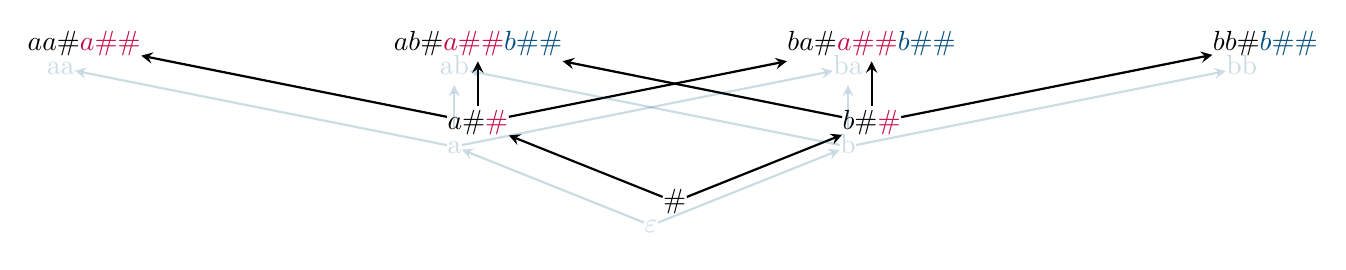
\begin{tikzpicture}[
        isWord/.style={rectangle,inner sep=0mm},
        isEmbedding/.style={->, >=stealth, thick},
        branch/.style={A5},
        antichain/.style={A2},
        branchEdge/.style={A5,dashed},
        outEdge/.style={dotted,B2},
        isInfixEnc/.style={},
        isRealWord/.style={A4,opacity=0.2},
        isRealEmbedding/.style={A4,opacity=0.2},
        isNewEdge/.style={B2},
        ]

\newcommand{\sep}[1]{\textcolor{gray}{\#^{#1}}}
\node[isWord,isInfixEnc] (Iepsilon) at (-4.7, 0.3) {\strut $\#$};
\node[isWord,isInfixEnc] (Ia) at (-7.2, 1.3) {\strut $a\#\textcolor{A2}{\#}$};
\node[isWord,isInfixEnc] (Ib) at (-2.2, 1.3) {\strut $b\#\textcolor{A2}{\#}$};
\node[isWord,isInfixEnc] (Iaa) at (-12.2, 2.3) {\strut $aa\#\textcolor{A2}{a\#\#}$};
\node[isWord,isInfixEnc] (Iab) at (-7.2, 2.3) {\strut $ab\#\textcolor{A2}{a\#\#}\textcolor{A4}{b\#\#}$};
\node[isWord,isInfixEnc] (Iba) at (-2.2, 2.3) {\strut $ba\#\textcolor{A2}{a\#\#}\textcolor{A4}{b\#\#}$};
\node[isWord,isInfixEnc] (Ibb) at (2.8, 2.3) {\strut $bb\#\textcolor{A4}{b\#\#}$};
\draw[isEmbedding] (Iepsilon) -- (Ia);
\draw[isEmbedding] (Iepsilon) -- (Ib);
\draw[isEmbedding] (Ia) -- (Iaa);
\draw[isEmbedding] (Ia) -- (Iab);
\draw[isEmbedding] (Ia) -- (Iba);
\draw[isEmbedding] (Ib) -- (Iab);
\draw[isEmbedding] (Ib) -- (Iba);
\draw[isEmbedding] (Ib) -- (Ibb);
\node[isWord,isInfixEnc,isRealWord] (epsilon) at (-5.0, 0) {\strut $\varepsilon$};
\node[isWord,isInfixEnc,isRealWord] (a) at (-7.5, 1) {\strut a};
\node[isWord,isInfixEnc,isRealWord] (b) at (-2.5, 1) {\strut b};
\node[isWord,isInfixEnc,isRealWord] (aa) at (-12.5, 2) {\strut aa};
\node[isWord,isInfixEnc,isRealWord] (ab) at (-7.5, 2) {\strut ab};
\node[isWord,isInfixEnc,isRealWord] (ba) at (-2.5, 2) {\strut ba};
\node[isWord,isInfixEnc,isRealWord] (bb) at (2.5, 2) {\strut bb};
\draw[isEmbedding,isRealEmbedding] (epsilon) -- (a);
\draw[isEmbedding,isRealEmbedding] (epsilon) -- (b);
\draw[isEmbedding,isRealEmbedding] (a) -- (aa);
\draw[isEmbedding,isRealEmbedding] (a) -- (ab);
\draw[isEmbedding,isRealEmbedding] (a) -- (ba);
\draw[isEmbedding,isRealEmbedding] (b) -- (ab);
\draw[isEmbedding,isRealEmbedding] (b) -- (ba);
\draw[isEmbedding,isRealEmbedding] (b) -- (bb);

\end{tikzpicture}
\end{document}
        
